% Gemini theme
% See: https://rev.cs.uchicago.edu/k4rtik/gemini-uccs
% A fork of https://github.com/anishathalye/gemini

\documentclass[final]{beamer}

% ====================
% Packages
% ====================

\usepackage[T1]{fontenc}
\usepackage{lmodern}
\usepackage[size=custom,width=120,height=72,scale=1.0]{beamerposter}
\usetheme{gemini}
% \usecolortheme{uchicago}
\usecolortheme{stanford}
\usepackage{graphicx}
\usepackage{booktabs}
\usepackage{tikz}
\usepackage{pgfplots}
\pgfplotsset{compat=1.17}

\usepackage[backend=biber,style=numeric, citestyle=ieee]{biblatex}
\addbibresource{egbib.bib} %Imports bibliography file

\graphicspath{{"../results/"}}

% ====================
% Lengths
% ====================

% If you have N columns, choose \sepwidth and \colwidth such that
% (N+1)*\sepwidth + N*\colwidth = \paperwidth
\newlength{\sepwidth}
\newlength{\colwidth}
\setlength{\sepwidth}{0.025\paperwidth}
\setlength{\colwidth}{0.3\paperwidth}

\newcommand{\separatorcolumn}{\begin{column}{\sepwidth}\end{column}}


\title{Minimal sampling for stochastic transmission economic assessment}


\author{Erich Trieschman \inst{1}}

\institute[shortinst]{\inst{1} Department of Statistics}

% ====================
% Footer (optional)
% ====================

\footercontent{
  \href{https://github.com/etrieschman}{github.com/etrieschman} \hfill
  CME364b Convex Optimization II, Spring 2023 \hfill
  \href{mailto:erich.j.trieschman@gmail.com}{etriesch@stanford.edu}}
% (can be left out to remove footer)

% ====================
% Logo (optional)
% ====================

% use this to include logos on the left and/or right side of the header:
% \logoright{
\includegraphics[height=7cm]{stanford_logos/Block_S_1_color_red.png}}
% \logoleft{\includegraphics[height=7cm]{logos/cs-logo-maroon.png}}

% ====================
% Body
% ====================

\begin{document}

% This adds the Logos on the top left and top right
\addtobeamertemplate{headline}{}
{
    \begin{tikzpicture}[remember picture,overlay]
    %   \node [anchor=north west, inner sep=3cm] at ([xshift=0.0cm,yshift=1.0cm]current page.north west)
    %   {\includegraphics[height=5.0cm]{stanford_logos/Stanford-CS.png}}; % uc-logo-white.eps
      \node [anchor=north east, inner sep=3cm] at ([xshift=0.0cm,yshift=2.5cm]current page.north east)
      {
\includegraphics[height=7.0cm]{stanford_logos/Block_S_1_color_red.png}};
    \end{tikzpicture}
}

\begin{frame}[t]
\begin{columns}[t]
\separatorcolumn

\begin{column}{\colwidth}
  \vspace*{-10}
  \begin{block}{Introduction}
    \textbf{Objective:} To minimize the number of samples needed for generating uncertainty bounds for transmission economic assessments
    \begin{itemize}
      \item Traditional transmission planning models use deterministic load and resource availability forecasts, neglecting uncertainty in assessing economic benefits.
      \item Transmission Economic Assessment Methodology (TEAM) offers a solution to address uncertainties by stress-testing transmission alternatives under future conditions in a stochastic production cost simulation. However, the simulations are computationally expensive.
      \item We develop methods to select minimal samples of load, wind, and solar forecasts for use in the TEAM framework; our methods leverage experiment design and active learning techniques. 
  \end{itemize}
  \end{block}

  \vspace*{-10}
  \begin{block}{Background: Production cost simulation and stochastic profiles}
    \begin{column}{0.25\colwidth}
      \vspace*{-10}
      \begin{figure}[h]
        \centering
        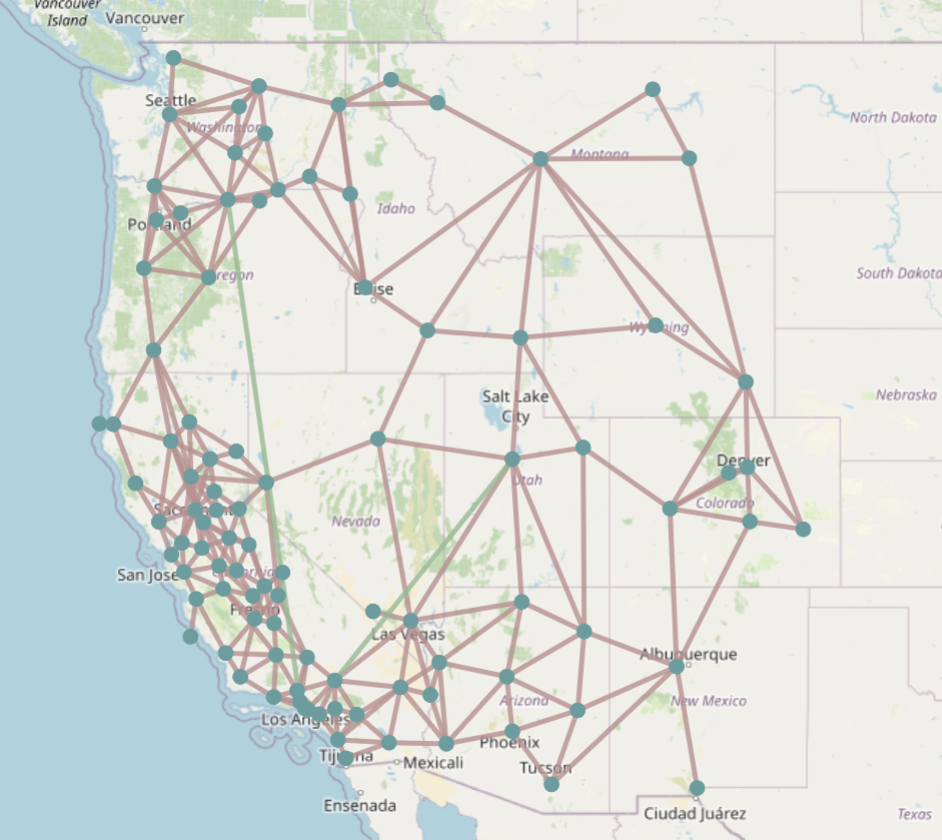
\includegraphics[scale=.5]{network.png}
        \caption{pypsa-usa 96-node WECC network}
      \end{figure}

    \end{column}
    \begin{column}{0.75\colwidth}
      \vspace*{-10}
    \begin{itemize}
      \item \textbf{Scenario:} We evaluate our methods under a single transmission expansion scenario for an HVDC VSC cable connecting Humboldt to PG\&E Bay in a synthetic 96-node network of the Western Electricity Coordinating Council (WECC).
      \begin{align*}
        \text{Benefits} &=  [\tilde{\lambda}_{n,t} - \lambda_{n,t}] \cdot P_{\text{load},n,t}
      \end{align*}
      \item \textbf{Cost model:} To estimate economic costs we use a nodal production cost simulation (PCS) model built on the Breakthrough Energy synthetic WECC network model. The WECC model is built within the Python for Power System Analysis (pypsa) toolkit. 
      \item \textbf{Stochastic profiles:} We generate stochastic load, wind, and solar profiles using the mean-reversion stochastic process method developed by the CAISO. Profiles are encoded using PCA to aid in sample selection; Only the first 10 principal components are used.
    \end{itemize}
    \end{column}
  \end{block}

  \vspace*{-10}
  \begin{block}{Methods}
    \begin{column}{0.7\colwidth}
      \begin{figure}[h]
        \centering
        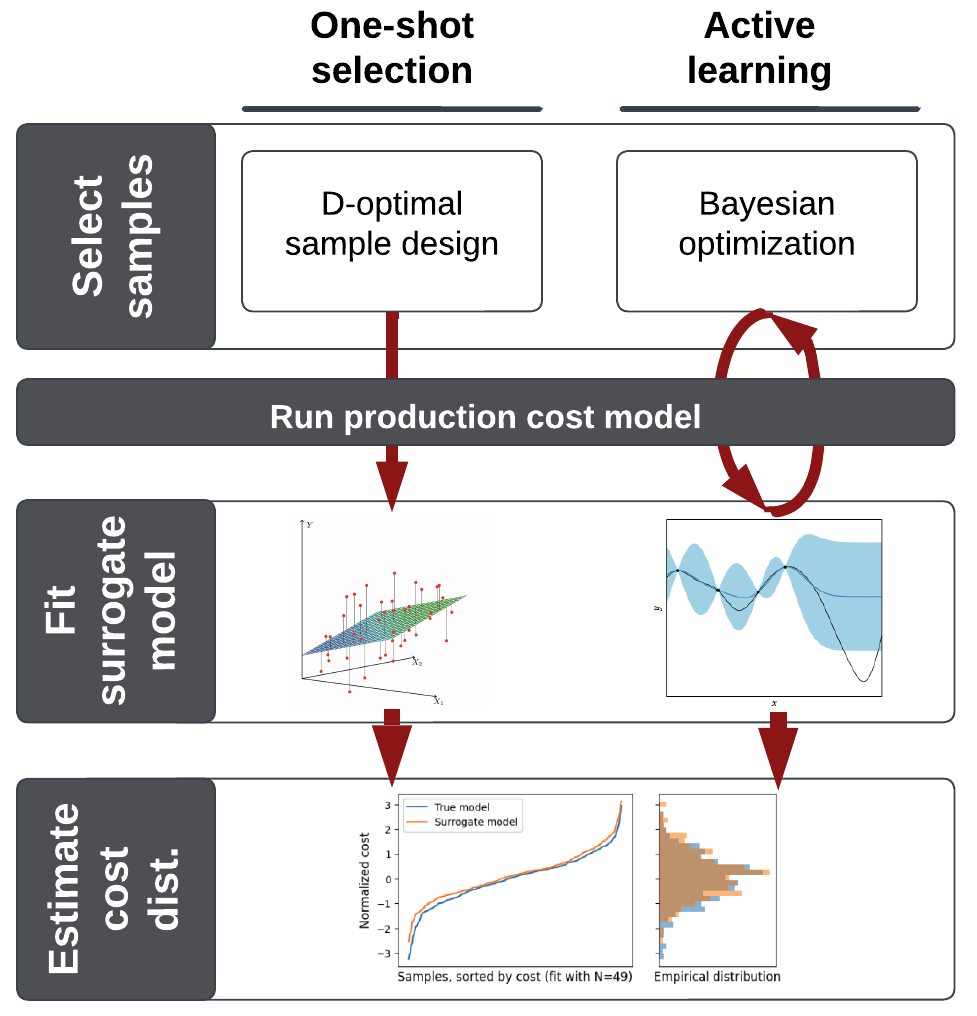
\includegraphics[scale=0.6]{methods_diagram.png}
      \end{figure}
\end{column}
\begin{column}{0.3\colwidth}
  \vspace*{-20}
  \begin{block}{Methods: Baselines}
    \begin{itemize}
      \item \textbf{Full sample:} Empirical distribution of the full sample of production cost model runs ($N=500$)
      \item \textbf{Random sample:} Empirical distribution generated by a surrogate model fit with randomly selected samples
      \item \textbf{Bootstrapping:} Bootstrapping used to generate confidence intervals around performance metrics
    \end{itemize}
  \end{block}
\end{column}
\end{block}
  
\end{column}

\separatorcolumn

\begin{column}{\colwidth}
  \vspace*{-10}
  \begin{block}{Methods: One-shot sample selection with D-optimal experiment design}    
    \begin{itemize}
      \item \textbf{Surrogate model:} Linear relationship between forecasts and costs
      \item \textbf{Objective:} Select samples that maximize forecast covariance matrix (equivalent to minimizing standard errors of $\hat{\beta}$). Use $m \in \{0, 1\}^n$ instead of the canonical formulation, $m \in \mathbb{Z}^n$, because the cost model is deterministic.
      \item \textbf{Convex relaxations:} Scalarize with D-optimal design formulation as described in Boyd et. al. and use L1-norm heuristics to maximize solution sparsity.
    \end{itemize}
    \begin{align*}
      \min_\lambda. \quad & -\log\det \left(\sum_{j=1}^p\lambda_jv_jv_j^T\right)\\
      s.t. \quad & 0 \preceq \lambda \preceq 1, \quad \lVert\lambda\rVert _1 \leq \alpha M
    \end{align*}
    For $p$ distinct forecasts, distinct scenario $v_j$, $m_j$ selecting scenario $v_j$, target scenarios $M$, and hyperparameter $\alpha$. This approach requires discretizing the dimensions of our input space $x_i$ into scenarios $v_j$.     

  \end{block}
  \vspace*{-10}
  \begin{block}{Methods: Active learning sample selection with Bayesian optimization}
    \begin{itemize}
      \item \textbf{Surrogate model:} Gaussian Process (GP) model
      \begin{align*}
        f^{(n+1)} \mid \textbf{x}^{(1:n+1)} \sim \mathcal{N}\left(\textbf{k}(x^{(n+1)})^T\textbf{K}^{-1}\textbf{f}^{(1:n)}, k(x^{(n+1)}, x^{(n+1)}) - \textbf{k}(x^{(n+1)})^T\textbf{K}^{-1}\textbf{k}(x^{(n+1)})\right)\\
        k(x^{(i)}, x^{(j)}) := \exp\left(-\frac{1}{2l^2}\lVert x^{(i)} - x^{(j)}\rVert^2_2\right) \quad 
        \textbf{k}(x^{(n+1)}) := \left[\dots, k(x^{(n+1)}, x^{(i)}), \dots\right] \quad
        \textbf{K}_{ij} := k(x^{(i)}, x^{(j)})
      \end{align*}

      \item \textbf{Objective:} Select the next sample point to maximize the entropy of the surrogate model fit to all previous samples. Maximum entropy search (MES) aims to reduce overall surrogate model uncertainty
      \begin{align*}
        &\; \textrm{argmax}_x \;\; \frac{1}{2}\log(2\pi k(x^{(n+1)}, x^{(n+1)}) - \textbf{k}(x^{(n+1)})^T\textbf{K}^{-1}\textbf{k}(x^{(n+1)})) + \frac{1}{2} = \; \textrm{argmin}_x \textbf{k}(x)^T\textbf{K}^{-1}\textbf{k}(x)
    \end{align*}

      \item \textbf{Convex relaxations:} Non-convex objective; Sequential convex programming (SCP) used to iteratively solve for local maxima for each sample, $x^{(n+1)}$
    \begin{align*}
        x^{(n+1)^{(k+1)}} &= \textrm{argmin}_x \hat{f}(x) \;\; \textrm{s.t} \;\; x \in \mathcal{T}^{(k)}
    \end{align*}

    \item \textbf{Function approximations:} Both second-order Taylor approximation and particle method approximation methods used to approximate the objective
    \vspace{10}
      \begin{itemize}
      \item \textbf{Second-order Taylor approximation:}
      \begin{align*}
        \hat{f}(x) = f(x^{(k)}) + \nabla f(x^{(k)})^T(x - x^{(k)}) + (x - x^{(k)})^T P (x - x^{(k)}) \textrm{ for } P = \left(\nabla^2 f(x^{(k)})\right)_+
      \end{align*}
      \item \textbf{Particle method approximation:} 
      \begin{align*}
        \hat{f}(x) &= (x - x^{(k)})^TP(x - x^{(k)}) + q^T(x - x^{(k)}) + r \textrm{ for}\\
        P, q, r &= \textrm{argmin}_{P\succeq 0, q, r} \sum_{i=1} \left((z_i - x^{(k)})^TP(x_i - x^{(k)}) + q^T(z_i - x^{(k)}) + r - f(z_i)\right)^2 \textrm{, for } z_i \sim \text{Unif}\left[\mathcal{T}^{(k)}\right]
      \end{align*}
      \end{itemize}
    \end{itemize}
  \end{block}
  
  \vspace*{-30}
  \begin{block}{Results}
    \begin{table}[h]
      \small
      \begin{center}
          \caption{\label{fig:summ} Absolute difference between true distribution and surrogate distribution statistic (samples=50, bootstraps=100)}
          \begin{tabular}{r|cc|ccc}
\toprule
 N=500& \multicolumn{2}{c|}{\textbf{One-shot selection}} & \multicolumn{3}{c}{\textbf{Active learning selection}} \\
 samples=50& Baseline & D-optimal & Baseline & Taylor & Particle \\
 \midrule
 Min        & 1.66±0.46   &  1.49     & 0.64 ± 0.53  &    0.46 ± 0.41  &   0.41 ± 0.39 \\
 5th pctl   & 0.87±0.28   &  0.85     & 0.68 ± 0.23  &    0.24 ± 0.16  &   0.23 ± 0.16 \\
 10th pctl  & 0.59±0.23   &  0.53     & 0.47 ± 0.19  &    0.14 ± 0.12  &   0.17 ± 0.14 \\
 25th pctl  & 0.32±0.16   &  0.26     & 0.28 ± 0.14  &    0.11 ± 0.10  &   0.14 ± 0.11 \\
 50th pctl  & 0.14±0.11   &  0.11     & 0.11 ± 0.09  &    0.09 ± 0.07  &   0.14 ± 0.10 \\
 75th pctl  & 0.31±0.16   &  0.34     & 0.26 ± 0.13  &    0.11 ± 0.09  &   0.12 ± 0.09 \\
 90th pctl  & 0.56±0.23   &  0.66     & 0.45 ± 0.17  &    0.14 ± 0.13  &   0.16 ± 0.12 \\
 95th pctl  & 0.62±0.27   &  0.75     & 0.47 ± 0.20  &    0.18 ± 0.17  &   0.18 ± 0.15 \\
 Max        & 1.34±0.52   &  1.35     & 0.76 ± 0.46  &    0.40 ± 0.45  &   0.53 ± 0.37 \\
 Mean       & 0.13±0.11   &  0.04     & 0.11 ± 0.09  &    0.09 ± 0.07  &   0.11 ± 0.09 \\
 Std        & 0.47±0.15   &  0.50     & 0.37 ± 0.09  &    0.10 ± 0.07  &   0.10 ± 0.07 \\
\bottomrule
\end{tabular}
      \end{center}
      \end{table}
    \end{block}


\end{column}

\separatorcolumn

\begin{column}{\colwidth}
  \vspace*{-10}
  \begin{block}{Results}

    \begin{column}{0.49\colwidth} 
      \vspace*{-20}
      \begin{block}{Active learning baseline}
      \begin{figure}[h]
          \centering
          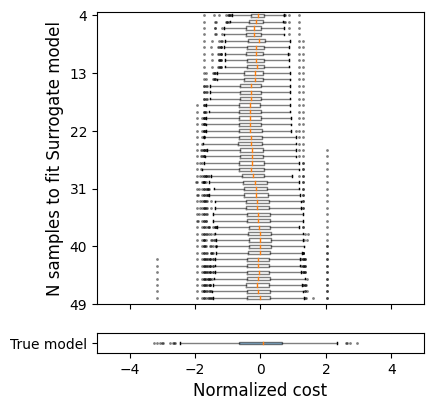
\includegraphics[scale=1.25]{rand_boxplot.png}
          % \caption{Random samples}
      \end{figure}
      \begin{figure}[h]
        \centering
        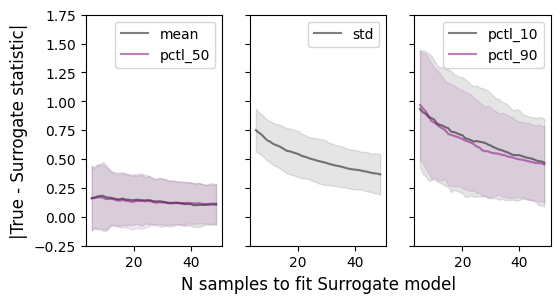
\includegraphics[scale=1]{rand_statsboot.png}
        % \caption{Random samples vs True samples}
    \end{figure}
  \end{block}
      \end{column}
      \begin{column}{0.49\colwidth} 
        \vspace*{-20}
        \begin{block}{Active learning Taylor approx.}
      \begin{figure}[h]
          \centering
          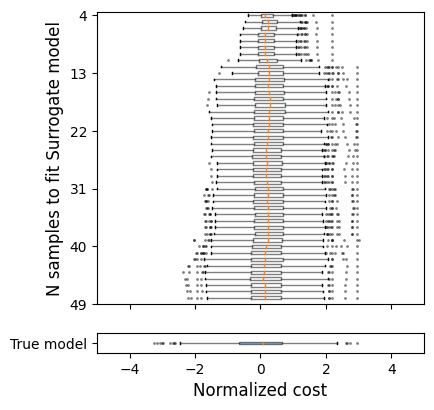
\includegraphics[scale=1.25]{taylor_boxplot.png}
          % \caption{Active learning samples}
      \end{figure}
      \begin{figure}[h]
        \centering
        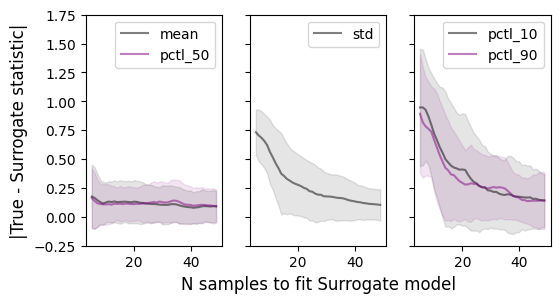
\includegraphics[scale=1]{taylor_statsboot.png}
        % \caption{Active learning samples vs. True samples}
    \end{figure}
  \end{block}
      \end{column}
      \footnotesize{Active learning samples selected with Taylor approximations in SCP. See final report appendix for the performance of the particle method and one-shot sample selection}

  \end{block}
  \vspace*{-10}
  \begin{block}{Discussion}
    \begin{itemize}
      \item Optimal sample selection methods can be used generate cost distributions at 5-10\% of the computational costs required to run the full production cost model for all samples
      \item Optimal sample selection methods outperform random sample selection methods, especially for estimating cost distribution percentiles and standard deviations.
      \item Active learning sample selection runtime is negligible compared to the production cost model runs (~30min); one-shot sample selection runtimes are on the order of minutes.
      \item \textbf{Future work:} Apply sampling method to general generation and transmission capacity expansion modeling (instead of a single-scenario assessment); improved hyperparameter tuning
  \end{itemize}

  \end{block}
  \vspace*{-10}
  \begin{block}{Contributions and acknowledgements}
    This work is conducted by Erich Trieschman as part of a larger project in collaboration with Kamran Tehranchi. Kamran is responsible for running the production cost model and generating stochastic profile data. Code and results are available on \href{https://github.com/etrieschman/grid-planner}{Github}.

  \end{block}
  \vspace*{-10}
  \begin{block}{References}
    \vspace*{-25}
    \nocite{boyd} \nocite{Rasmussen} \nocite{zhang_using_2010}
    \tinysize{\printbibliography[heading=none]}
  \end{block}

\end{column}

\separatorcolumn
\end{columns}
\end{frame}

\end{document}
